%%%%%%%%%%%%%%%%%%%%%%%%%%%%%%%%%%%%%%%%%
%
% (c) 2022 by Jennifer Laaser
%
% This work is licensed under the Creative Commons Attribution-NonCommercial-ShareAlike 4.0 International License. To view a copy of this license, visit http://creativecommons.org/licenses/by-nc-sa/4.0/ or send a letter to Creative Commons, PO Box 1866, Mountain View, CA 94042, USA.
%
% The current source for these materials is accessible on Github: https://github.com/jlaaser/pogil-polymers
%
%%%%%%%%%%%%%%%%%%%%%%%%%%%%%%%%%%%%%%%%%

\renewcommand{\figpath}{content/polymchem/stepgrowth/kinetics/figs}
\renewcommand{\labelbase}{step-kinetics}

\begin{activity}{Kinetics of Step-Growth Polymerizations}

\begin{instructornotes}

	This activity introduces students to key concepts related to the kinetics of step-growth polymerizations.
	
	After completing this activity, students will be able to:
			\begin{enumerate}
				\item \dots
			\end{enumerate}
	
			
	\subsection*{Activity summary:}
	\begin{itemize}
		\item \textbf{Activity type:} Learning Cycle
		\item \textbf{Content goals:} See above
		\item \textbf{Process goals:} %https://pogil.org/uploads/attachments/cj54b5yts006cklx4hh758htf-process-skills-official-pogil-list-2015-original.pdf
			\begin{itemize}
				%\item Linking concepts to derive a key result
				\item Written and oral communication of reasoning
			\end{itemize}
		\item \textbf{Duration:} TBD %approx. 45 minutes
		\item \textbf{Instructor preparation required:} none beyond knowledge of relevant content
		\item \textbf{Related textbook chapters:}
			\begin{itemize}
				\item \emph{Polymer Chemistry} (Hiemenz \& Lodge), 2nd ed.: sections 2.2.3 and 2.3
				\item \emph{Introduction to Polymers} (Young \& Lovell), 3rd ed.: \dots 
			\end{itemize}
	\end{itemize}

\end{instructornotes}

	%\textbf{Focus question:} Put a central question for the students to consider through this exercise here.

\begin{model}[A Simple Step-Growth Reaction]
\label{\labelbase:mdl:simple}

	The key reaction in a step-growth polymerization is the reaction of an ``A'' functional group with a ``B'' functional group to form an ab bond:
	
	\centerline{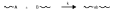
\includegraphics[width=0.7\textwidth]{\figpath/Model1_rxn}}
	
	The rate of this reaction is determined by the rate constant $k$.

\end{model}


\begin{ctqs}

	\question How many molecules must come together for this reaction to take place?
	
		\begin{solution}[0.5in]
			2
		\end{solution}
	
	\question Based on your answer to the previous question, explain, in 1-2 complete sentences, why it is appropriate to describe this reaction as a \emph{bimolecular} reaction.
	
		\begin{solution}[1in]
			Bimolecular reactions are reactions in which two molecules come together to participate in a reaction.  Because two reactant molecules participate in this reaction, it is bimolecular.
		\end{solution}
	
	\question Propose an appropriate expression describing how the rate at which ``A'' reactive groups are used up depends on the rate constant and the concentrations of both reactive species.
		\label{\labelbase:ctq:proposeratelaw}
		
		\begin{solution}[1in]
			\begin{equation*}
				\frac{d[A]}{dt} = -k[A][B]
			\end{equation*}
			(negative because A groups are used up as the reaction progresses)
		\end{solution}
		
\end{ctqs}

\begin{infobox}
	It is possible to show (see Exercise \ref{\labelbase:exc:catinteratelaw}) that, if the reaction is stoichiometrically balanced and has an initial concentration of ``A'' groups of $[A]_0$, the concentration of unreacted ``A'' groups changes as
	\begin{equation*}
		[A] = \frac{[A]_0}{1 + k[A]_0 t}
	\end{equation*}	
	with time.
	\label{\labelbase:infobox:catintegrated}
\end{infobox}

\begin{ctqs}

	\question Using this information, derive appropriate expressions describing how...
	
		\begin{enumerate}
			\item ... the extent of reaction, $p$, changes with time:
			
				\begin{solution}[2.5in]
					The extent of reaction is the fraction of A groups that \emph{have} reacted.  If the initial concentration of A groups was $[A]_0$ and the current concentration of A groups is $[A]$, then the concentration that have reacted is $[A]_0 - [A]$ and the fraction that have reacted is this number divided by the original number, or
					
					\begin{align*}
						p &= \frac{[A]_0-[A]}{[A]_0} \\
						  &= 1 - \frac{[A]}{[A]_0}\\
						  &= 1- \frac{1}{1 + k[A]_0 t}
					\end{align*}
				\end{solution}
			
			\item ... the number-average degree of polymerization, $N_n$, changes with time: \label{\labelbase:ctq:catNn}
			
				\begin{solution}[2in]
					\begin{align*}
						N_n &= \frac{1}{1-p}\\
							&= \frac{1}{1-\left(1- \frac{1}{1 + k[A]_0 t}\right)}\\
							&= \frac{1}{\frac{1}{1 + k[A]_0 t}}\\
							&= 1 + k[A]_0 t
					\end{align*}
				\end{solution}
			
		\end{enumerate}
	
	\question Based on the equation you derived above, sketch a plot of how the molecular weight of the polymers you expect to obtain in a step-growth reaction will change with time:
	
		\centerline{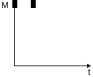
\includegraphics[width=0.4\textwidth]{\figpath/Model1_axes}}

\end{ctqs}
	

\begin{model}[Kinetics of Esterification Reactions]
\label{\labelbase:mdl:esterification}

	Esterification reactions used in polymer synthesis often proceed by the following mechanism (a Fischer esterification):
	
	\centerline{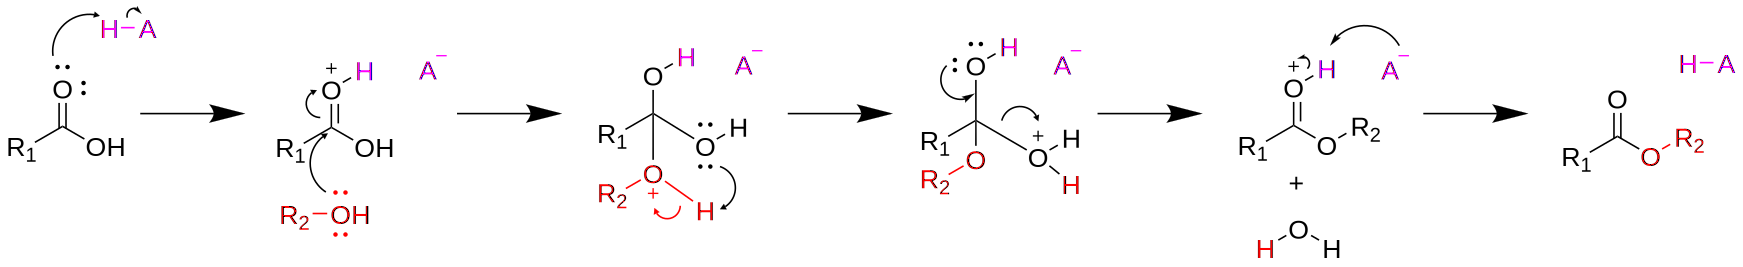
\includegraphics[width=\textwidth]{\figpath/Model2_mechanism}}

\end{model}

\begin{ctqs}

		\question In Activity 3.\ref{stepgrowth-chem}, you learned that esterification reactions typically require a carboxylic acid (R-COOH) and an alcohol (R-OH).  What \emph{additional} chemical species is required for the mechanism shown in Model \ref{\labelbase:mdl:esterification}?
		
			\begin{solution}[0.5in]
				An acid, H-A
			\end{solution}
		
		\question What happens to this additional reagent over the course of the reaction shown in Model \ref{\labelbase:mdl:esterification}?
		
			\begin{solution}[1.25in]
				It protonates the carboxylic acid, but is regenerated at the end of the mechanism (it is not used up or permanently bonded to the products).
			\end{solution}
		
		\question Based on your answer to the previous two questions, explain, in 1-2 complete sentences, why this reaction is referred to as an \emph{acid-catalyzed} esterification.
		
			\begin{solution}[1.75in]
			\end{solution}
			
		\question How many different molecules must come together for this reaction to proceed?
		
			\begin{solution}[0.5in]
			\end{solution}
		
		\question Explain, in 1-2 complete sentences, why the kinetics of this reaction should obey
		
			\begin{equation*}
				\frac{d[\text{COOH}]}{dt} = - k \text{[COOH][OH][HA]}
			\end{equation*}
			
			where [COOH], [OH], and [HA] are the concentrations of the carboxylic acid, alcohol, and acid catalyst, respectively.\label{\labelbase:ctq:fisherratelaw}
			
				\begin{solution}[2.5in]
				\end{solution}
		
\end{ctqs}

\begin{infobox}
	In Fisher esterifications such as the reaction shown in Model \ref{\labelbase:mdl:esterification}, the acidic protons required to catalyze the reaction can be supplied either by an added acid, such as sulfuric acid, or by other carboxylic acids present in the reaction mixture.
\end{infobox}

\begin{ctqs}
	
	\question When the acidic proton is supplied by an added acid, we refer to the polymerization as a ``catalyzed'' step-growth polymerization.
	
		\begin{enumerate}
			\item Briefly explain why, in this case, it is reasonable to assume that [HA] is constant over the entire course of the reaction.
			
				\begin{solution}[1.5in]
				\end{solution}
			
			\clearpage
			\item Critique or defend the following statement in 2-3 complete sentences:
			
				``The rate law for a catalyzed step-growth polymerization can effectively be simplified to $\frac{d[COOH]}{dt} = - k_c [COOH][OH]$, and the degree of polymerization grows linearly with time as in the bimolecular reaction shown in Model \ref{\labelbase:mdl:simple}.''
			
				\begin{solution}[2in]
				
				TRUE - if [HA] is constant then we can just let $k_c = k[HA]$ and the expression from CTQ 10 just reduces to the expression given in the statement.
				
				\end{solution}
				
		\end{enumerate}
		
	\question When the acidic proton is supplied by COOH groups from other monomers in the reaction mixture, we refer to the polymerization as an ``uncatalyzed'' step-growth polymerization.
	
		\begin{enumerate}
				
			\item  What rate law do you obtain if you replace [HA] in the expression given in CTQ \ref{\labelbase:ctq:fisherratelaw} with [COOH]?
			
				\begin{solution}[0.5in]	
					\begin{equation*}
						\frac{d[\text{COOH}]}{dt} = - k \text{[COOH]}^2\text{[OH]}
					\end{equation*}
				\end{solution}
		
			\item What happens to the concentration of COOH groups as the reaction progresses?
			
				\begin{solution}[0.5in]	
					[COOH] decreases as COOH groups are used up to form ester bonds.
				\end{solution}
			
			\item Based on your answers to the previous two questions, what do you expect to happen to the reaction rate as the reaction progresses?
			
				\begin{solution}[0.5in]	
					Because the rate depends on the square of the COOH concentration, the reaction rate will slow down substantially as the concentration of COOH groups decreases.
				\end{solution}
			
		\end{enumerate}
	
\end{ctqs}

\begin{infobox}\label{\labelbase:info:uncatintrate}
	The integrated rate law for uncatalyzed step-growth polymerizations is
	\begin{equation*}
		\frac{1}{[A]^2} = 2k_u t + \frac{1}{[A]_0^2}
	\end{equation*}
	which can be rewritten in terms of the extent of reaction as
	\begin{equation*}
		\frac{1}{(1-p)^2} = 1 + 2k_u [A]_0^2 t
	\end{equation*}
\end{infobox}

\begin{ctqs}

	\question Using this information, find an expression for how the number average degree of polymerization, $N_n$, changes with time in a self-catalyzed step-growth polymerization.
	
		\begin{solution}[1in]
			\begin{equation*}
				N_n = \sqrt{1 + 2k_u [A]_0^2 t}
			\end{equation*}
		\end{solution}
		
	\question Based on the equation you derived above, sketch a plot of how the molecular weight of the polymers you expect to obtain in a step-growth reaction will change with time:
	
		\centerline{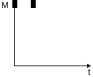
\includegraphics[width=0.4\textwidth]{\figpath/Model1_axes}}
		
	\question Which type of polymerization (catalyzed or uncatalyzed) do you expect to produce higher molecular weight polymers in a given amount of time?  Explain your group's reasoning in 2-3 complete sentences.
	
		\begin{solution}[2in]
		\end{solution}

\end{ctqs}
	

\begin{exercises}

		\exercise In Model \ref{\labelbase:mdl:simple}, the ``A'' and ``B'' reactive groups were shown without depicting what species they were attached to.  However, these species could be on the ends of monomers, oligomers, or long polymer chains. %add graphic?
		What assumption has to be made about the reactivities of the functional groups on these different species for the rate law you proposed in CTQ \ref{\labelbase:ctq:proposeratelaw} (and the expression you derived for $N_n$ in CTQ \ref{\labelbase:ctq:catNn}) to correctly describe the kinetics of the entire reaction?  Explain your reasoning in 2-3 complete sentences.
			
		\exercise Derive the integrated rate law for stoichiometrically-balanced, catalyzed step-growth polymerizations (shown on page \pageref{\labelbase:infobox:catintegrated}) by doing the following: \label{\labelbase:exc:catinteratelaw}
		
			\begin{enumerate}
				\item Explain why, if the reaction is stoichiometrically balanced, it must be true that $[A]=[B]$ throughout the \emph{entire} course of the reaction.  Then, use this information to rewrite your expression from CTQ \ref{\labelbase:ctq:proposeratelaw} in terms of the concentration of A groups only.
				
				\item Rearrange your equation into the form $f([A])\,d[A] = g(t)\,dt$ and then integrate both sides.
				
				\item Finally, apply the initial condition that $[A]=[A]_0$ at $t=0$ and show that your answer rearranges to the form shown in the Information box on page \pageref{\labelbase:infobox:catintegrated}.
			\end{enumerate}
			
		\exercise Extend the process from the above question to derive...
			
			\begin{enumerate}
				\item ... the rate law for stoichiometrically-balanced, un-catalyzed step-growth polymerizations (shown on page \pageref{\labelbase:info:uncatintrate}).
				
				\item ... the rate law for a stoichiometrically-\emph{unbalanced} catalyzed step-growth polymerization that starts with A and B reactive group concentrations of $[A]_0$ and $[B]_0$, respectively.
			\end{enumerate}
			
		%\exercise The kinetic scheme shown in Model \ref{\labelbase:mdl:simple} is somewhat over-simplified.  In practice, most step-growth reactions can be thought of as proceeding through formation of a ``caged'' intermediate, where the A and B reactive groups 
		
\end{exercises}
	
\end{activity}